% ====================================================
%  LLM 互联接口产品线调研 — Beamer 模版
%  Author: 葛良晨
%  Date:   2026-05-27
%  Compile: latexmk -xelatex -shell-escape
% ====================================================
\documentclass[aspectratio=169, 10pt, UTF8]{ctexbeamer}

% ---------- 主题与颜色 ----------
\usetheme{Madrid}
\usecolortheme{default}

\definecolor{ieeeBlue}{RGB}{0, 83, 159}
\definecolor{ieeeRed}{RGB}{198, 38, 46}
\definecolor{ieeeGreen}{RGB}{0, 114, 41}
\definecolor{ieeeOrange}{RGB}{235, 110, 31}
\definecolor{darkGray}{RGB}{66, 66, 66}

\setbeamercolor{structure}{fg=ieeeBlue}
\setbeamercolor{alerted text}{fg=ieeeRed}
\setbeamercolor{example text}{fg=ieeeGreen}
\setbeamercolor{frametitle}{bg=ieeeBlue!15, fg=ieeeBlue}
\setbeamercolor{block title}{bg=ieeeBlue!15, fg=ieeeBlue}
\setbeamercolor{block body}{bg=ieeeBlue!5}
\setbeamercolor{block title example}{bg=ieeeGreen!15, fg=ieeeGreen}
\setbeamercolor{block body example}{bg=ieeeGreen!5}
\setbeamercolor{block title alerted}{bg=ieeeRed!15, fg=ieeeRed}
\setbeamercolor{block body alerted}{bg=ieeeRed!5}

% ---------- 包 ----------
\usepackage{graphicx}
\usepackage{booktabs}
\usepackage{tabularx}
\usepackage{multirow}
\usepackage[table]{xcolor}
\usepackage{amsmath,amssymb}
\usepackage{tikz}
\usetikzlibrary{positioning, calc, shapes.geometric, arrows.meta, backgrounds, fit, shadows}
\usepackage{hyperref}

% ---------- 页脚 ----------
\setbeamertemplate{footline}[frame number]

% ---------- 每节前显示目录 ----------
\AtBeginSection[]{
  \begin{frame}{本节内容}
    \tableofcontents[currentsection]
  \end{frame}
}

% ---------- 元信息 ----------
\title[LLM 互联接口产品线调研]{LLM 互联接口具体产品线调研}
\subtitle{竞品分析 · 技术路线 · 市场定位}
\author[葛良晨]{葛良晨}
\institute[]{}
\date{\today}

\begin{document}

% ============================================
%  标题页
% ============================================
\begin{frame}
  \titlepage
\end{frame}

% ============================================
%  目录
% ============================================
\begin{frame}{汇报大纲}
  \tableofcontents
\end{frame}

% ================================================================
\section{调研背景与目标}
% ================================================================

\begin{frame}{调研背景}
  \begin{block}{行业背景}
    \begin{itemize}
      \item
    \end{itemize}
  \end{block}

  \begin{alertblock}{核心问题}
    \begin{itemize}
      \item
    \end{itemize}
  \end{alertblock}
\end{frame}

\begin{frame}{调研范围与方法}
  \begin{columns}[T]
    \begin{column}{0.50\textwidth}
      \begin{block}{覆盖产品线}
        \begin{itemize}
          \item
          \item
          \item
        \end{itemize}
      \end{block}
    \end{column}
    \begin{column}{0.50\textwidth}
      \begin{exampleblock}{评估维度}
        \begin{itemize}
          \item 技术指标
          \item 市场定位
          \item 竞争格局
          \item 供应链成熟度
        \end{itemize}
      \end{exampleblock}
    \end{column}
  \end{columns}
\end{frame}

% ================================================================
\section{产品线总览}
% ================================================================

\begin{frame}{产品线全景图}
  \centering
  % 示例：产品矩阵 TikZ 图
\end{frame}

\begin{frame}{产品线分类矩阵}
  \centering
  \footnotesize
  \begin{tabularx}{\textwidth}{p{2.4cm} p{2.8cm} p{3.2cm} p{3.2cm} p{3.0cm}}
    \toprule
    \textbf{产品类别} & \textbf{代表厂商} & \textbf{核心指标} & \textbf{目标场景} & \textbf{成熟度} \\
    \midrule
    Retimer / Redriver
      & 澜起(M88RT6), Astera(Aries), 谱瑞
      & 64 GT/s, 43 dB
      & AI 服务器, AEC, 存储
      & PCIe 6.x 送样 \\
    \addlinespace
    智能线缆 (AEC)
      & 澜起(2026.01), Astera(Taurus)
      & 800G PAM4
      & 机架内 ToR-NIC
      & 澜起新发布 \\
    \addlinespace
    交换芯片
      & Astera(Scorpio), 芯动
      & 32--320 Lanes
      & GPU 集群组网
      & 国产早期 \\
    \addlinespace
    CXL 内存控制器
      & 澜起(MXC), Astera(Leo)
      & CXL 3.1, 2 TB
      & 内存池化, KVCache
      & 澜起领跑 \\
    \addlinespace
    SuperNIC
      & Enfabrica(ACF-S)
      & 3.2 Tbps
      & 多协议融合
      & 海外 C 轮 \\
    \addlinespace
    D2D PHY IP
      & Eliyan(NuLink)
      & 224 Gbps/lane
      & Chiplet 互联
      & 海外融资 \\
    \addlinespace
    硅光 / CPO
      & Ayar, Celestial
      & 8 Tbps CPO
      & 光互联终局
      & 海外 E 轮 \\
    \bottomrule
  \end{tabularx}
\end{frame}

% ================================================================
\section{物理层：Retimer 与 Smart Cable 产品线}
% ================================================================

\begin{frame}{澜起科技 M88RT61632 — 核心规格}
  \centering
  \begin{columns}[T]
    \begin{column}{0.42\textwidth}
      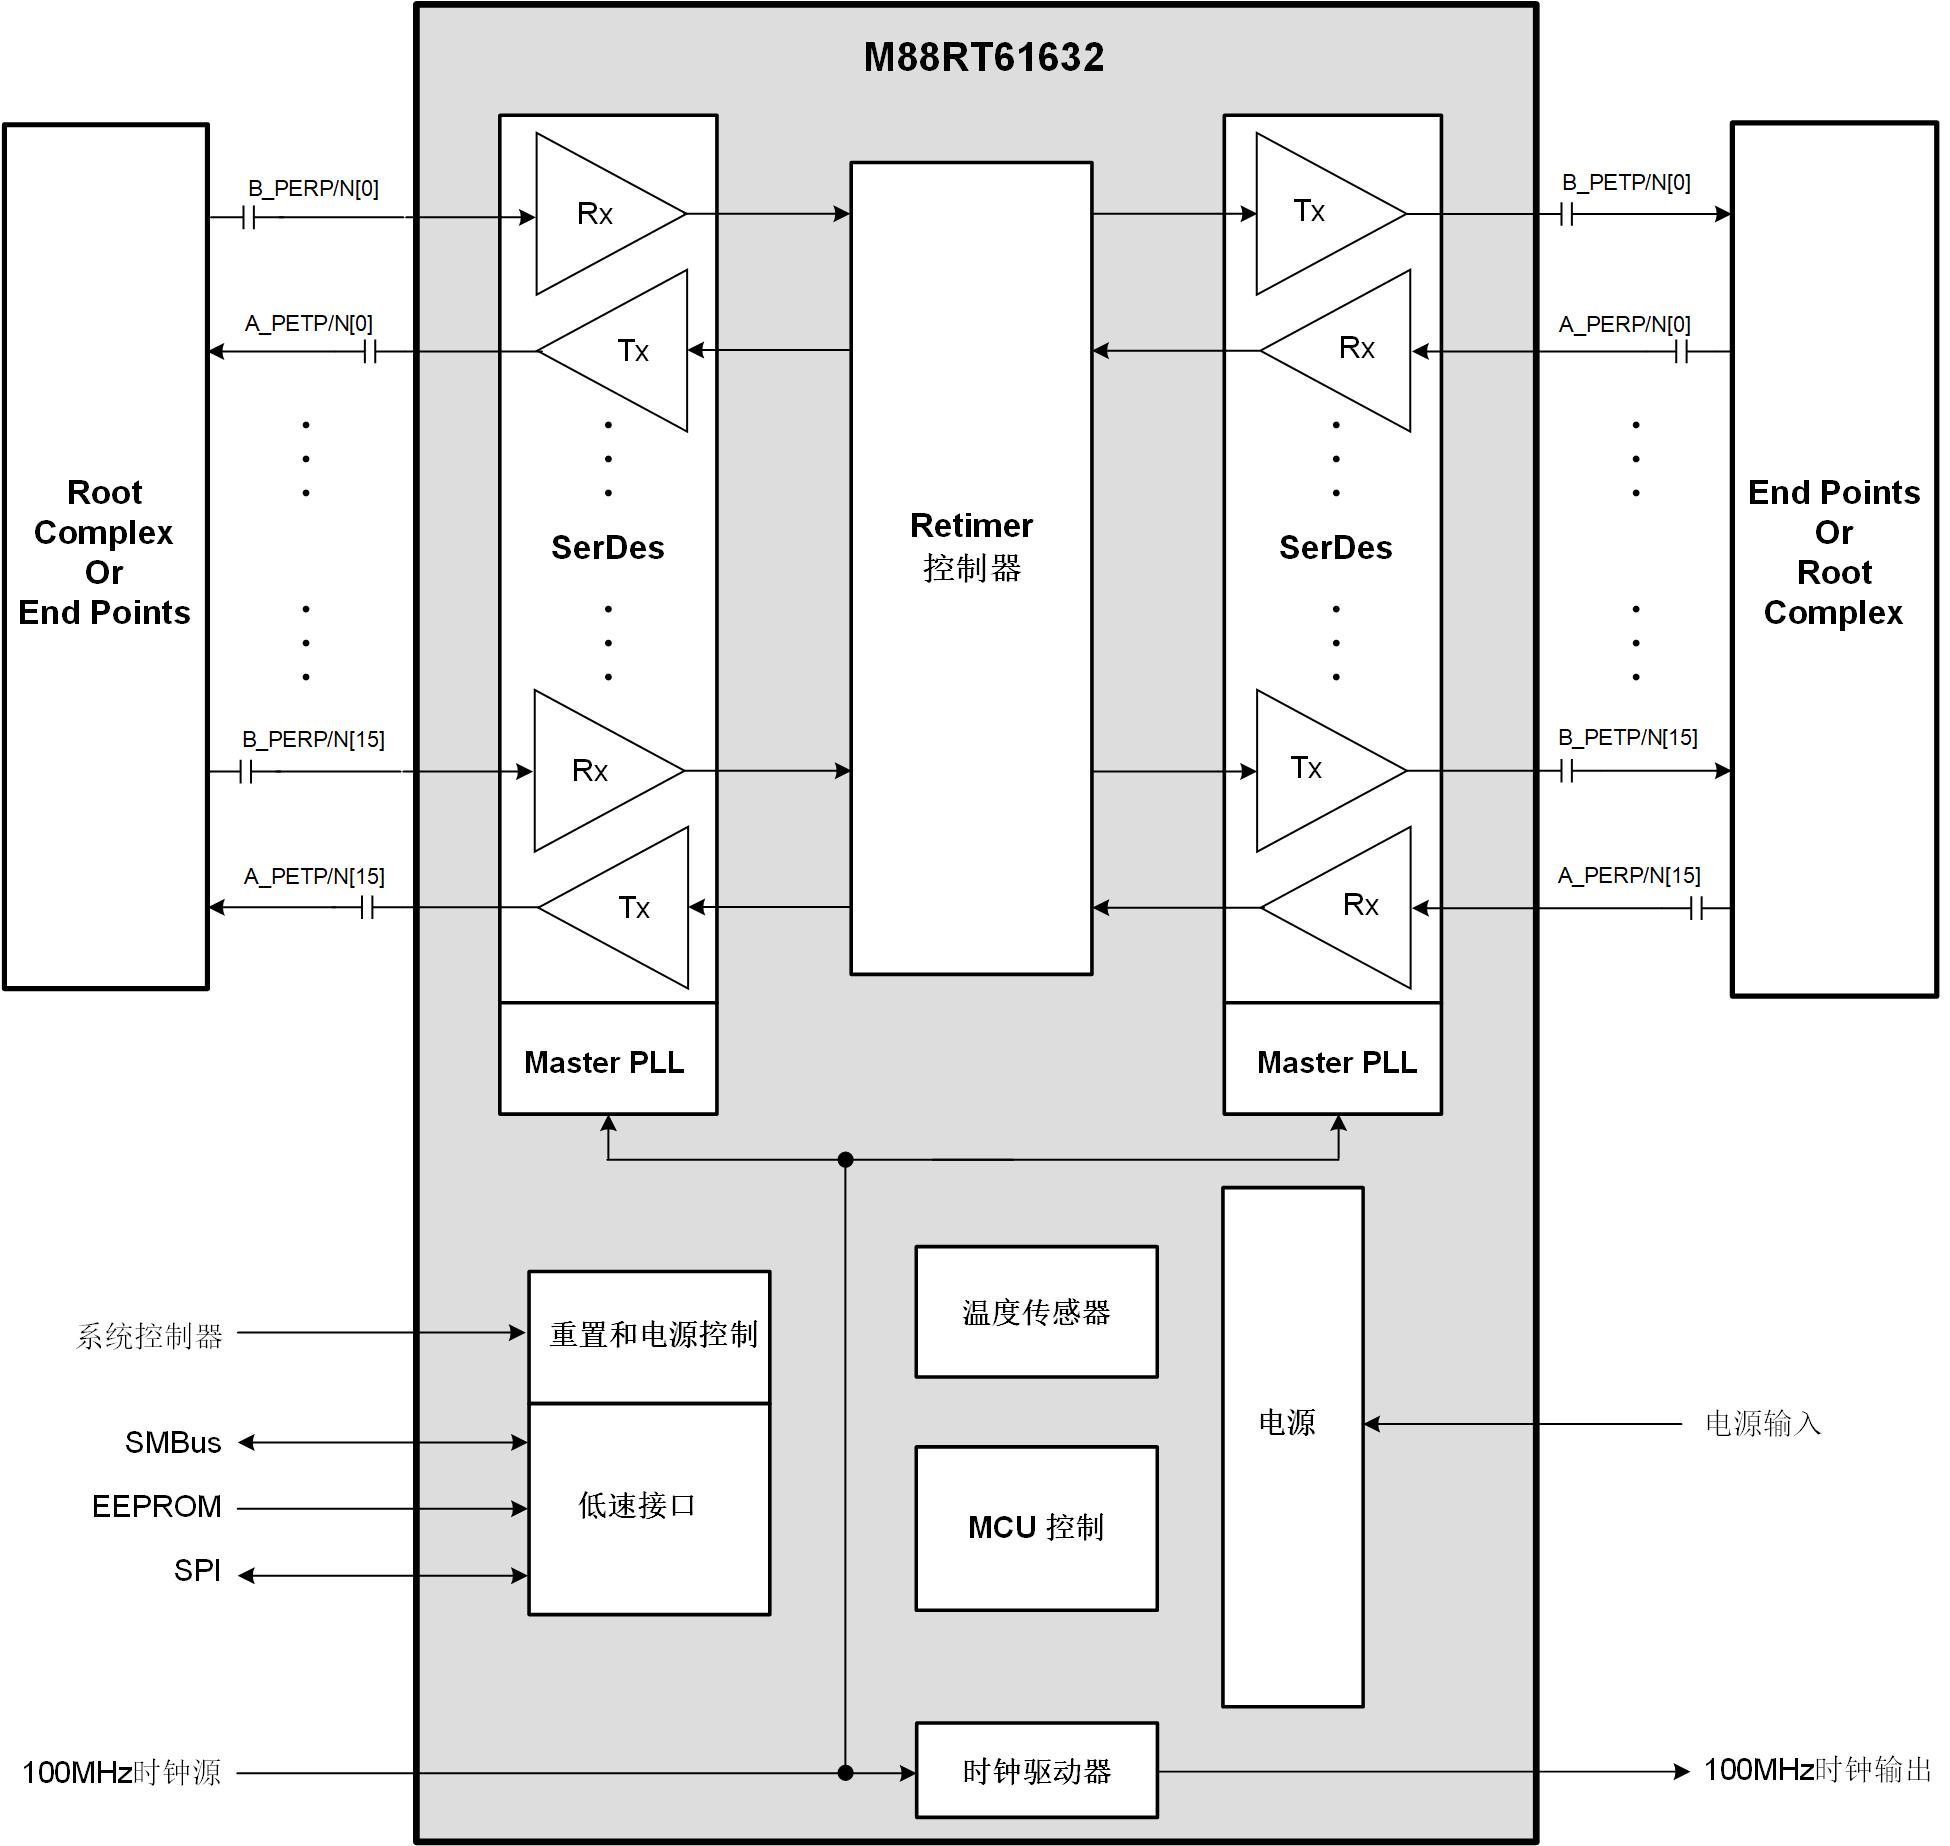
\includegraphics[width=\textwidth]{M88RT61632_Block_Diagram.jpg}
      \vspace{4pt}
      {\footnotesize 来源：澜起科技官网}
    \end{column}
    \begin{column}{0.58\textwidth}
      \begin{block}{M88RT61632 (2025.01 送样)}
        \begin{itemize}
          \item 16 通道 PCIe 6.x / CXL 3.x Retimer
          \item 最大速率 \textbf{64 GT/s}（自研 PAM4 SerDes）
          \item 链路预算补偿 \textbf{高达 43 dB}
          \item 354-ball FCCSP 业界主流封装
          \item 分叉：1×16, 2×8, 4×4, 最多 8×2
          \item 向下兼容 64/32/16/8/5/2.5 GT/s
          \item L0P / L1PM 低功耗模式
          \item SMBus / I3C 管理 + SPI/EEPROM 固件
        \end{itemize}
      \end{block}
    \end{column}
  \end{columns}
\end{frame}

\begin{frame}{澜起 Retimer 产品线全貌}
  \begin{block}{技术演进路线}
    \centering
    \footnotesize
    \begin{tabularx}{\textwidth}{p{3.2cm} p{1.8cm} p{4.5cm} p{3.5cm}}
      \toprule
      \textbf{产品代} & \textbf{状态} & \textbf{关键指标} & \textbf{市场地位} \\
      \midrule
      PCIe 4.0 Retimer & 已量产 & — & 进入较晚，份额较小 \\
      \addlinespace
      PCIe 5.0 / CXL 2.0 & 已量产 & 32 GT/s，出货\textbf{超百万颗} (2024) & 全球第 2，市占率 \textbf{\textasciitilde10.9\%} \\
      \addlinespace
      \textbf{PCIe 6.x / CXL 3.x} & \textbf{送样中} & \textbf{M88RT61632}, 64 GT/s, 43 dB & 全球第 2 家推出 \\
      \addlinespace
      PCIe 7.0 Retimer & 研发中 & 128 GT/s 目标 & 与 Astera 同步研发 \\
      \addlinespace
      PCIe Switch & 研发中 & — & 国内空白填补 \\
      \addlinespace
      以太网 PHY Retimer & 研发中 & — & 新赛道布局 \\
      \bottomrule
    \end{tabularx}
  \end{block}

  \vspace{6pt}
  \begin{alertblock}{核心壁垒}
    自研 64 GT/s PAM4 SerDes IP — 国内极少数掌握该核心技术的厂商
  \end{alertblock}
\end{frame}

\begin{frame}{代表产品对比：澜起 vs Astera Labs vs 谱瑞}
  \centering
  \footnotesize
  \begin{tabularx}{\textwidth}{p{2.4cm} X X X}
    \toprule
    \textbf{指标} & \textbf{澜起 M88RT61632} & \textbf{Astera Aries (PCIe 6)} & \textbf{谱瑞 PS8926} \\
    \midrule
    速率      & \textbf{64 GT/s} PAM4     & 64 GT/s PAM4               & 32 GT/s (PCIe 5.0) \\
    通道数    & 16                        & 16                         & 16 \\
    链路预算  & \textbf{高达 43 dB}        & \textasciitilde36 dB        & \textasciitilde36 dB \\
    协议      & PCIe 6.x / CXL 3.x        & PCIe 6.x / CXL 3.x         & PCIe 5.0 / CXL 2.0 \\
    制程      & —                         & —                          & — \\
    SerDes    & \textbf{自研} PAM4 IP       & 自研 DSP                    & 自研 \\
    封装      & 354-ball FCCSP             & 小型封装                     & 业界主流 \\
    送样时间  & 2025.01                   & 2024 (业界首家)              & 已量产 \\
    低功耗    & L0P + L1PM                & 低功耗设计                   & 支持 \\
    管理      & SMBus / I3C              & SMBus                       & SMBus \\
    软件生态  & GUI + SDK                & \textbf{COSMOS} 遥测套件     & 基础工具 \\
    \bottomrule
  \end{tabularx}

  \vspace{6pt}
  \begin{alertblock}{关键差距}
    Astera 先发 \textbf{\textasciitilde10 个月}，COSMOS 软件生态构成最大护城河；澜起在链路预算 (43 dB) 上反超。
  \end{alertblock}
\end{frame}

\begin{frame}{技术壁垒与市场格局}
  \begin{columns}[T]
    \begin{column}{0.50\textwidth}
      \begin{block}{硬件壁垒}
        \begin{itemize}
          \item \textbf{SerDes IP}：64 GT/s PAM4 高速串行接口设计，国内仅澜起等极少数掌握
          \item \textbf{信号完整性验证}：43 dB 链路预算下 DSP 均衡、DFE、CDR 综合调优
          \item \textbf{互操作性认证}：跨 CPU/GPU/SSD/NIC 多厂商兼容性测试矩阵
          \item \textbf{PCI-SIG 合规}：PCIe 6.0 认证流程复杂，周期长
        \end{itemize}
      \end{block}
    \end{column}
    \begin{column}{0.50\textwidth}
      \begin{alertblock}{生态壁垒}
        \begin{itemize}
          \item \textbf{COSMOS 软件}：Astera 的遥测/诊断/OTA 套件是真正护城河
          \item \textbf{客户绑定}：Astera 已深度集成 NVIDIA/AWS/Meta 系统
          \item \textbf{先发时间差}：Astera 领先 \textasciitilde10 个月量产 PCIe 6.0
          \item \textbf{固件迭代}：大规模部署中的 bug 修复和性能调优需要时间积累
        \end{itemize}
      \end{alertblock}
    \end{column}
  \end{columns}

  \vspace{8pt}
  \begin{exampleblock}{市场格局 (2024)}
    \centering
    全球 PCIe Retimer 市场：Astera \textbf{\textasciitilde86\%} \quad 澜起 \textbf{\textasciitilde10.9\%} \quad 其他 \textasciitilde3\%
    \quad$\to$\quad 两家合计占据 \textbf{96.9\%} 市场份额
  \end{exampleblock}
\end{frame}

\begin{frame}{澜起科技：财务表现与战略定位 (2025 年报)}
  \begin{columns}[T]
    \begin{column}{0.48\textwidth}
      \begin{block}{2025 年核心财务数据}
        \begin{itemize}
          \item 总营收 \textbf{54.56 亿元} (+49.9\% YoY)
          \item 归母净利润 \textbf{22.36 亿元} (+58.4\%)
          \item 互连类芯片收入 \textbf{51.39 亿元} (+53.4\%)，占 94.2\%
          \item 互连芯片毛利率 \textbf{65.6\%}
          \item 2026E 券商预测营收 75.07 亿 (+37.6\%)
          \item 2027E 预测营收 95.62 亿，净利 44.70 亿
        \end{itemize}
      \end{block}
    \end{column}
    \begin{column}{0.52\textwidth}
      \begin{exampleblock}{战略卡位}
        \begin{itemize}
          \item \textbf{国内唯一} 在 Retimer + CXL MXC + AEC 全面对标 Astera 的厂商
          \item 内存接口芯片 (RCD/DB/MRCD/MDB/CKD) 全球市占率 \textasciitilde45\%
          \item 「内存互连 + 高速运力」双轮驱动
          \item CXL 3.1 MXC 芯片已送样，部分节点 \textbf{全球领跑}
          \item PCIe 7.0 Retimer 工程研发积极推进
          \item 以太网 PHY Retimer + Switch 新赛道布局
        \end{itemize}
      \end{exampleblock}

      \vspace{6pt}
      \begin{alertblock}{与 Astera 的差距}
        Astera 2025 全年收入 \$8.525 亿 (+115\%)，净利润 \$2.19 亿，市值 \textasciitilde\$230 亿。澜起市值 \textasciitilde2200 亿 RMB，体量接近但 Retimer 市占率差距显著。
      \end{alertblock}
    \end{column}
  \end{columns}
\end{frame}

\begin{frame}{澜起 PCIe 6.x/CXL 3.x AEC 有源电缆方案 (2026.01)}
  % 缩小此 frame 的正文字体，使用局部字号命令，避免影响全局模板。
  % 常用 LaTeX 字号命令（由小到大）：
  %   \tiny, \scriptsize, \footnotesize, \small, \normalsize, \large, \Large, \LARGE, \huge, \Huge
  % 约略对应点数（以文档基准 10pt 为例，仅供参考）：
  %   \tiny=5pt, \scriptsize=7pt, \footnotesize=8pt, \small=9pt, \normalsize=10pt,
  %   \large=12pt, \Large=14.4pt, \LARGE=17.28pt, \huge=20.74pt, \Huge=24.88pt
  % 在 Beamer 中常用做法：在单个 frame 内使用局部字号（如 \small / \footnotesize）
  % 以减小该帧正文的字体；避免在浮动体或复杂盒子内频繁切换字号。
  % 选择 \footnotesize 作为折衷（比默认小一号，但仍可读）。
  \footnotesize
  \centering
  \begin{columns}[T]
    \begin{column}{0.38\textwidth}
      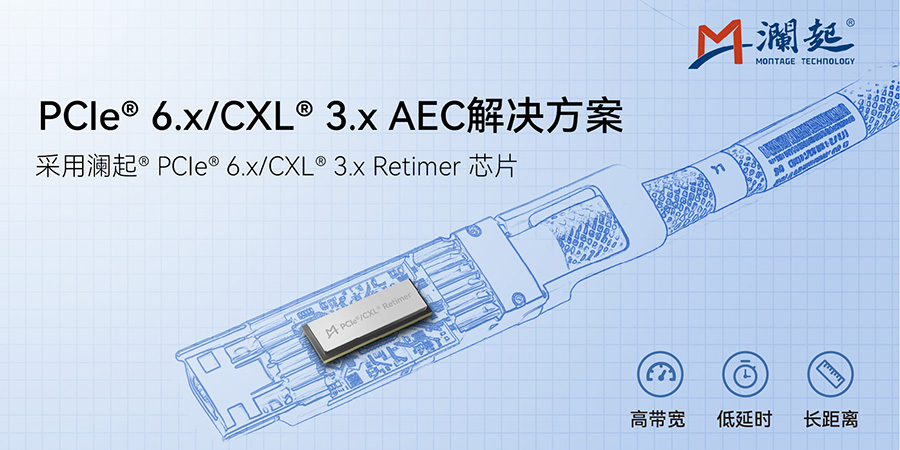
\includegraphics[width=\textwidth]{PCIe6_AEC_product.jpg}
      \vspace{6pt}
      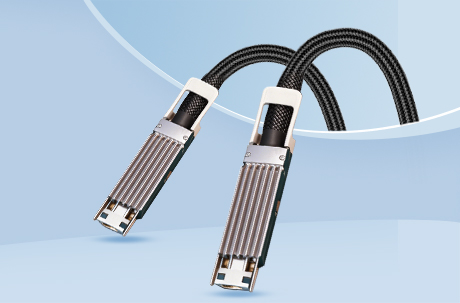
\includegraphics[width=\textwidth]{PCIe6.0AEC.jpg}
    \end{column}
    \begin{column}{0.62\textwidth}
      \vspace{-10pt}
      \begin{block}{产品概况}
        \begin{itemize}
          \item 2026.01.26 发布，\textbf{国内率先}推出 PCIe 6.x/CXL 3.x AEC
          \item 采用自研 Retimer 芯片 + SerDes + DSP 架构
          \item 接口封装：\textbf{OSFP-XD} 高密度接头
          \item 支持 PCIe 6.0 x16 高速稳定传输
          \item 内置链路监控与诊断功能
          \item 多种线缆规格，适配机箱内/外、跨板卡、机柜间等场景
        \end{itemize}
      \end{block}

      \vspace{-5pt}
      \begin{exampleblock}{关键进展}
        \begin{itemize}
          \item 已与 CPU、xPU、PCIe Switch、网卡完成 \textbf{互操作测试}
          \item 与国内多家主流线缆厂商 \textbf{联合开发及系统验证}
          \item 对标 Astera Taurus (800G 以太网 AEC)
        \end{itemize}
      \end{exampleblock}

      \vspace{-5pt}
      \begin{alertblock}{战略意义}
        Retimer 芯片 + AEC 线缆 = 从芯片到系统的垂直整合。以低于光模块的成本和功耗，实现 PCIe 6.0 长距信号延展，填补 \textbf{中短距高速互连} 市场空白。
      \end{alertblock}
    \end{column}
  \end{columns}
\end{frame}

\begin{frame}{AEC 产业链格局与速率演进}
  \centering
  \begin{columns}[T]
    \begin{column}{0.98\textwidth}
      \begin{block}{产业链双层结构}
        \textbf{互连与线缆方案大厂：}
        \begin{itemize}
          \item \textbf{Credo}：AEC 先驱，主导 HiWire 联盟，既做芯片也出成品，微软/亚马逊核心供应商
          \item \textbf{Amphenol / Molex}：互连连接器全球巨头，与多家芯片厂合作，产品线最全
          \item \textbf{FS (飞速) / Approved Networks}：面向数据中心和 AI 集群的定制化高性价比方案
        \end{itemize}
        \vspace{4pt}
        \textbf{核心芯片 (Retimer / DSP) 供应商：}
        \begin{itemize}
          \item \textbf{Marvell / Broadcom}：网络芯片双雄，DSP 广泛集成于安费诺/莫仕 AEC 接头内部
          \item \textbf{Astera Labs / Point2}：专注高速互连信号调理 (PCIe 5.0, 112G/224G)
        \end{itemize}
      \end{block}
      \begin{alertblock}{AEC vs DAC vs AOC 核心区别}
        \textbf{DAC (无源)}：极低成本，但 800G 时距离被压缩至 2.5m 内，无法跨机柜。\\
        \textbf{AEC (有源)}：两端内嵌 Retimer 芯片 (CDR + 均衡)，功耗 6{\textasciitilde}12W，距离延伸至 7m。\\
        \textbf{AOC (有源光缆)}：距离最长 (>100m)，成本最高，功耗最大。
      \end{alertblock}
    \end{column}
  \end{columns}

\end{frame}

\begin{frame}{AEC 速率与距离演进趋势}
  \vspace{-3pt}
  \centering
  \footnotesize

  \begin{tabularx}{\textwidth}{c c c c}
    \toprule
    \textbf{聚合总速率} & \textbf{单通道信号速率} & \textbf{AEC 最大传输距离} & \textbf{常见接口封装} \\
    \midrule
    400G  & 56G PAM4   & \textbf{可达 7 米}   & QSFP56, QSFP-DD, OSFP \\
    800G  & 112G PAM4  & \textbf{5{\textasciitilde}7 米} & QSFP112, QSFP-DD, OSFP \\
    1.6T  & 224G PAM4  & \textbf{2.5{\textasciitilde}3 米} & OSFP, OSFP-XD \\
    \bottomrule
  \end{tabularx}

  \vspace{6pt}
  \begin{center}
    \textbf{AEC 填补了短距铜缆 (DAC) 与长距光纤 (AOC) 之间的关键空白 — 400G/800G 已大规模商用，1.6T 进入量产初期}
  \end{center}

  \begin{columns}[T]
    \begin{column}{0.98\textwidth}
      % 在此插入两张并排图片（占列宽各 48%），替换文件名为实际图片路径。
      \vspace{6pt}
      \begin{center}
        \begin{minipage}[b]{0.28\textwidth}
          \centering
          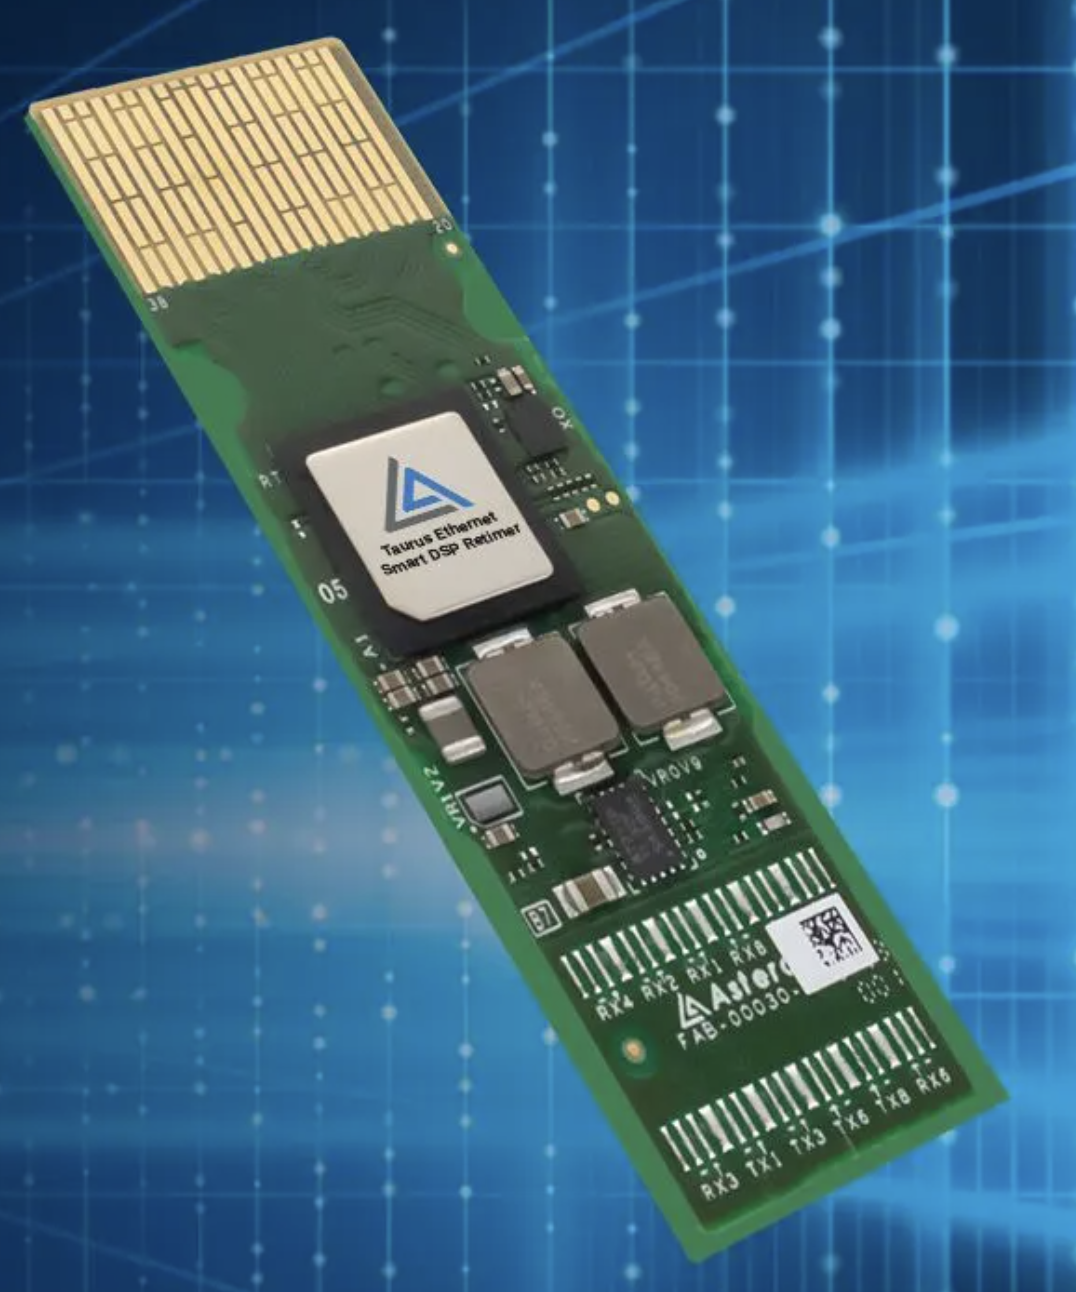
\includegraphics[width=\linewidth]{taurus.png} % <-- 替换为实际图片文件名
        \end{minipage}\hfill
        \begin{minipage}[b]{0.28\textwidth}
          \centering
          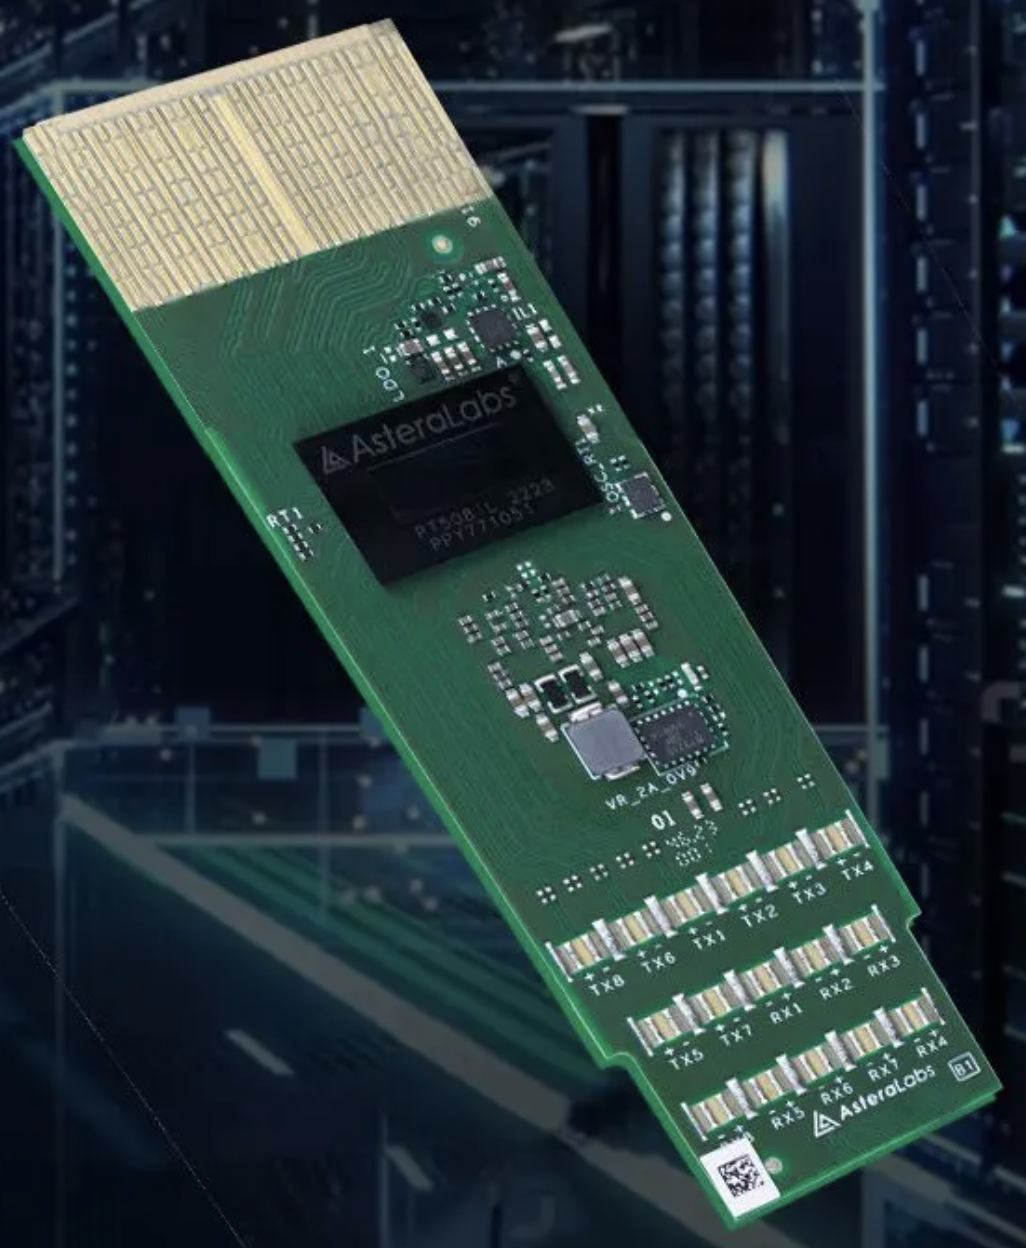
\includegraphics[width=\linewidth]{aries_scm.png} % <-- 替换为实际图片文件名
        \end{minipage}
      \end{center}
    \end{column}
  \end{columns}
\end{frame}

\begin{frame}{Astera Labs Aries Smart Cable Module — 产品规格}
  \centering
  \scriptsize
  \begin{columns}[T]
    \begin{column}{0.48\textwidth}
      \begin{block}{产品定义与定位}
        \begin{itemize}
          \item Aries Retimer IC + 外围组件集成于 paddle card，嵌入 AEC 线缆两端
          \item 支持直连电缆 (Straight) 和扇出电缆 (Breakout) 形态
          \item 目标场景：Server-to-JBOG / JBOG-to-JBOG / Switch-to-JBOG
          \item 实现 PCIe 6.0 x16 在细径铜缆上的长距稳定传输
        \end{itemize}
      \end{block}
      \vspace{-10pt}
      \begin{alertblock}{物理性能}
        \begin{itemize}
          \item PCIe 5.0：最远 \textbf{7 米}，多种铜缆规格
          \item PCIe 6.x：最远 \textbf{6 米}，细径铜缆
          \item 支持 64/32/8/5/2.5 GT/s，\textbf{自动链路均衡}
          \item 灵活分叉：1×16, 2×8, 4×4, 8×2 等
        \end{itemize}
      \end{alertblock}
    \end{column}
    \begin{column}{0.48\textwidth}
      \begin{exampleblock}{高级特性}
        \begin{itemize}
          \item \textbf{自动方向检测}：对称电缆设计，即插即用
          \item \textbf{自动极性校正} + Lane Reversal 支持
          \item SRIS / SRNS 时钟拓扑
          \item 支持热插拔 (Hot Plug / Hot Un-plug)
          \item 接收端 Lane Margining (时序 + 电压)
          \item 协议层 Loopback + PRBS 生成/检查
          \item 低功耗先进 CMOS 工艺 + L1.0 低功耗模式
          \item \textbf{不停机固件升级} (Non-disruptive FW Update)
        \end{itemize}
      \end{exampleblock}
    \end{column}
  \end{columns}

  \vspace{4pt}
  \centering
  \footnotesize
  \begin{tabularx}{\textwidth}{p{2.0cm} p{2.2cm} p{2.2cm} p{3.0cm} p{3.0cm}}
    \toprule
    \textbf{料号系列} & \textbf{PCIe 代} & \textbf{通道数} & \textbf{量产状态} & \textbf{备注} \\
    \midrule
    PM20-5xx & PCIe 5.0 & 多种配置 & \textbf{量产 (Production)} & 2025.04 产品手册发布 \\
    PM30-6xx & PCIe 6.x & 多种配置 & \textbf{预量产 (Pre-Prod)} & 向下兼容全部前代 \\
    \bottomrule
  \end{tabularx}

  \vspace{4pt}
  \begin{center}
    \textbf{COSMOS 遥测套件}：实时监控眼图张开度、均衡器水平、结温等，可配置中断告警。Full C/Python SDK，加速故障隔离。
  \end{center}
\end{frame}

\begin{frame}{Astera Labs Taurus Smart Cable Module — 以太网 AEC}
  \centering
  \scriptsize
  \vspace{-10pt}
  \begin{columns}[T]
    \begin{column}{0.48\textwidth}
      \begin{block}{产品定义与定位}
        \begin{itemize}
          \item 面向 \textbf{以太网 Scale-Out} 场景的有源铜缆模块 (ACC)
          \item 集成于 QSFP-DD / QSFP-DD800 / OSFP 标准接口
          \item 替代粗重无源 DAC 和高成本 AOC，填充 3m 内成本最优区间
          \item 支持 200G / 400G / \textbf{800G} 三代速率
        \end{itemize}
      \end{block}
      \vspace{-10pt}
      \begin{alertblock}{物理性能}
        \begin{itemize}
          \item 线速率：100G PAM4 / 50G PAM4 / 25G NRZ
          \item 最远 \textbf{3 米} (30/32/34 AWG 细径铜缆)
          \item 端到端延迟 \textbf{< 100 ns}
          \item 功耗比 AOC 低 \textbf{高达 50\%}
          \item 支持 PTP 精密时钟协议的 fanout 缓冲
        \end{itemize}
      \end{alertblock}
    \end{column}
    \begin{column}{0.48\textwidth}
      \begin{exampleblock}{高级特性与安全}
        \begin{itemize}
          \item 每通道独立控制：速率 / PAM4-NRZ / 聚合-解聚模式
          \item \textbf{深度线缆诊断}：眼图指标读出、PRBS 误码率、loopback
          \item 安全固件加载 + 非授权访问防护
          \item \textbf{不停机固件升级} (最高 1 MHz I\textsuperscript{2}C)
          \item 符合 CMIS 通用管理接口规范
        \end{itemize}
      \end{exampleblock}

    \vspace{4pt}
    \begin{center}
      \textbf{应用场景}：ToR Switch \\ $\updownarrow$ \\Server NIC (X-DAC) $\cdot$ ToR Switch \\ $\updownarrow$ \\ Leaf Switch (Straight) $\cdot$ ToR Switch Breakout $\to$ 多 Server NIC
      \end{center}
    \end{column}

  \end{columns}

  \vspace{4pt}
  \centering
  \scriptsize
  \begin{tabularx}{\textwidth}{p{1.0cm} p{2.6cm} p{2.2cm} p{3.2cm} p{3.4cm}}
    \toprule
    \textbf{总速率} & \textbf{料号} & \textbf{封装} & \textbf{线速率} & \textbf{距离 / 线规} \\
    \midrule
    200G & EM200-QDX-A & QSFP-DD   & 25G 或 50G/Lane & 3m 34AWG / 3m 32AWG \\
    400G & EM400-QDX-A & QSFP-DD   & 50G 或 100G/Lane & 3m 32AWG / 3m 30AWG \\
    400G & EM400-EPS-A & OSFP      & 50G 或 100G/Lane & 3m 32AWG / 3m 30AWG \\
    800G & EM800-QDX-A & QSFP-DD   & 100G/Lane       & 3m 30AWG \\
    800G & EM800-EPS-A & OSFP      & 100G/Lane       & 3m 30AWG \\
    \bottomrule
  \end{tabularx}


\end{frame}

% ================================================================
\section{交换层：Smart Switch / Fabric 产品线}
% ================================================================

\begin{frame}{PCIe Switch：LLM 万卡集群的「超级立交桥」}
  \scriptsize
  \begin{columns}[T]
    \begin{column}{0.52\textwidth}
      \begin{block}{市场格局：从垄断到国产突围}
        \begin{itemize}
          \item \textbf{国际巨头}：博通 (Broadcom) + 微芯 (Microchip) 长期垄断中高端，博通在 AI 服务器占据绝对主导
          \item \textbf{Astera Labs}：Scorpio 系列在 PCIe/CXL 交换 + Retimer 全球领先
          \item \textbf{国产破局}：2025{\textasciitilde}2026 成为「落地元年」，PCIe 5.0 世代密集突破流片 + 商用部署
        \end{itemize}
      \end{block}
      \begin{alertblock}{三大核心应用场景}
        \begin{enumerate}
          \item \textbf{GPU 高速互联}：CPU/GPU/NIC/NVMe 间动态调度，消除带宽瓶颈，支持 All-Reduce 参数同步
          \item \textbf{资源池化 (CDI)}：物理分区/虚拟化灵活分配 GPU/存储给不同宿主机
          \item \textbf{对等通信 (NTB)}：GPU Direct，绕过 CPU 直接读写 NVMe 或 GPU-GPU 通信
        \end{enumerate}
      \end{alertblock}
    \end{column}
    \begin{column}{0.48\textwidth}
      \begin{exampleblock}{技术演进四方向}
        \textbf{1. 大通道 + 高速率}
        \begin{itemize}
          \item 主流切换 PCIe 5.0 (32 GT/s)，96→104→\textbf{120} Lane
          \item 前瞻 PCIe 6.0/7.0：112G/224G SerDes + PAM4
        \end{itemize}
        \textbf{2. 系统级互联架构}
        \begin{itemize}
          \item 自研 FabricLink 等高级路由，万卡级无损对等互连
        \end{itemize}
        \textbf{3. CXL 深度融合}
        \begin{itemize}
          \item 集成 CXL 2.0/3.0 控制器，实现内存池化 + 缓存一致性
        \end{itemize}
        \textbf{4. 全栈自研 IP}
        \begin{itemize}
          \item 摆脱海外第三方 IP，MAC + SerDes PHY 完全自主正向设计
        \end{itemize}
      \end{exampleblock}
    \end{column}
  \end{columns}
\end{frame}

\begin{frame}{国内代表企业对比}
  \centering
  \footnotesize
  \begin{tabularx}{\textwidth}{p{2.0cm} p{3.0cm} p{4.0cm} p{3.5cm}}
    \toprule
    \textbf{公司} & \textbf{核心产品} & \textbf{进展 (截至 2026)} & \textbf{生态与合作} \\
    \midrule
    \textbf{芯动科技} & GX9120: 120 通道 PCIe 5.0 & 2026.02 首发, 115ns 延迟, 16 卡全互联 & 国产主流服务器适配导入 \\
    \addlinespace
    \textbf{数渡科技} & 104 通道 PCIe 5.0 Switch & 2026 初批量部署，落地联通星罗京津冀平台 & 深度绑定华为昇腾 (910B/950)，授权 FabricLink \\
    \addlinespace
    \textbf{井芯微电子} & JXW8848 全国产自主 Switch & 2025 下半年量产，全链路自主可控 & AI 智算中心 + 高安全等级设备 \\
    \addlinespace
    \textbf{澜起科技} & PCIe 5.0/6.0 Retimer & Retimer 细分赛道全球领先 & 配合 PCIe Switch 解决信号完整性问题 \\
    \bottomrule
  \end{tabularx}

  \vspace{6pt}
  \begin{center}
    \textbf{万通发展 2025 下半年斥巨资控股数渡科技 — 资本市场对国产高速互联芯片赛道高度认可}
  \end{center}
\end{frame}

\begin{frame}{芯动科技 GX9120 — 全球首款 120 通道 PCIe Gen5 Switch}
  \centering
  \begin{columns}[T]
    \begin{column}{0.38\textwidth}
      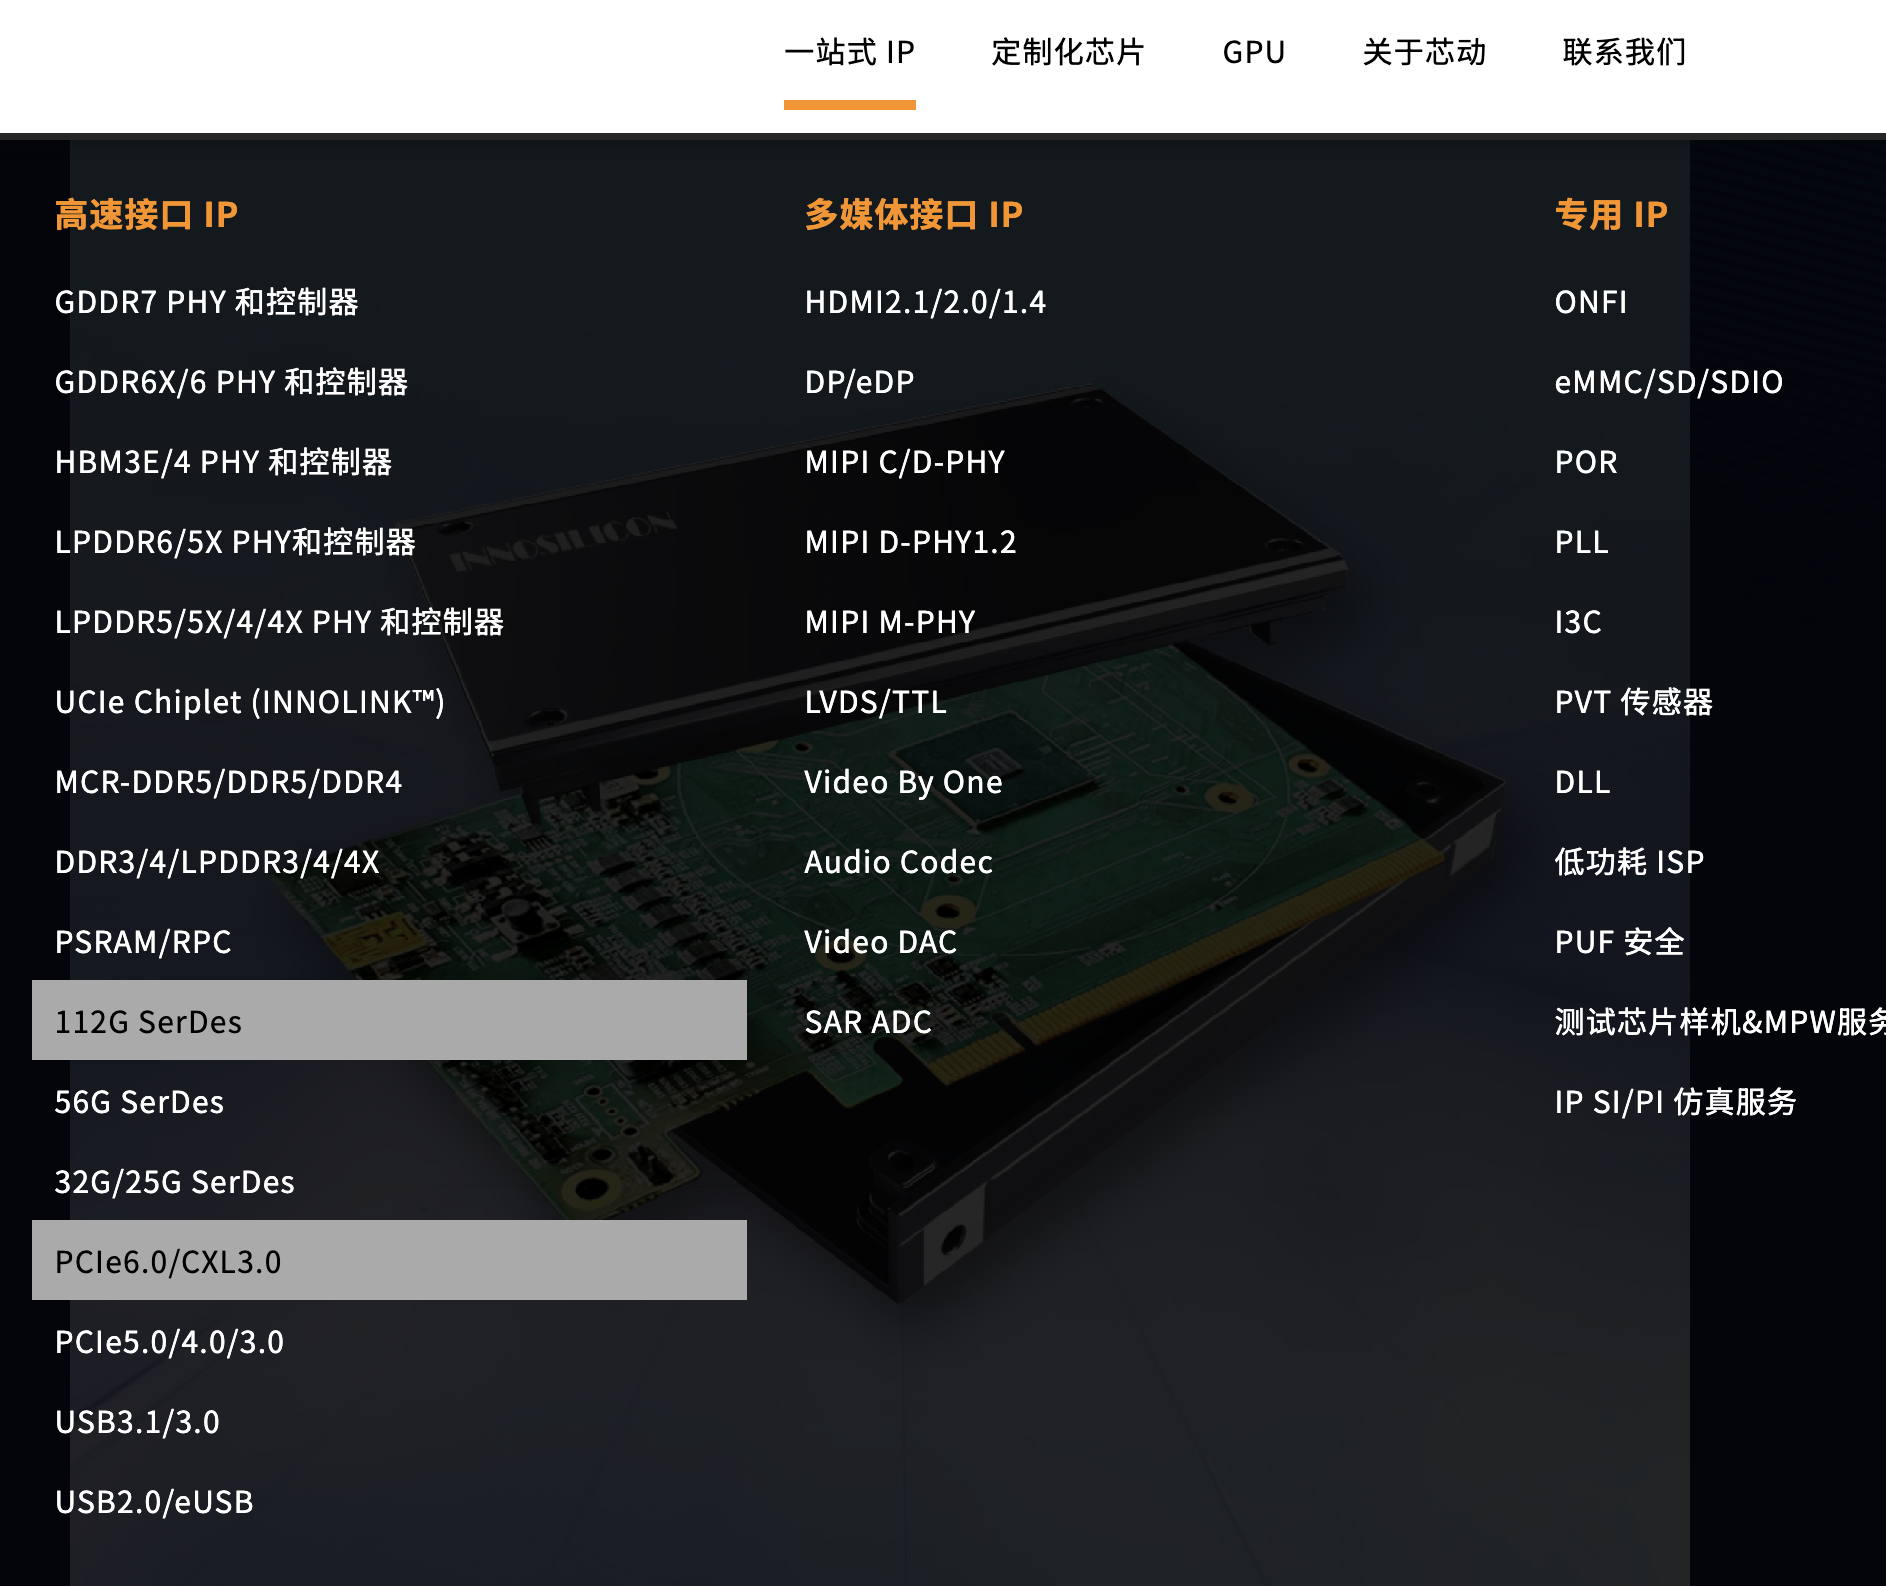
\includegraphics[width=\textwidth]{innosilicon_ip.png}
      \vspace{4pt}
      {\footnotesize 来源：芯动科技官网}
    \end{column}
    \begin{column}{0.62\textwidth}
      \begin{block}{GX9120 核心规格 (2026.02 武汉光谷发布)}
        \begin{itemize}
          \item \textbf{120} 条 PCIe Gen5 通道，30 个可灵活配置端口
          \item 单通道 \textbf{32 GT/s}，全交叉非阻塞交换架构
          \item 超低延迟：\textbf{115 ns}（纳秒级）
          \item SerDes：多级 FFE + 自适应 CTLE + \textbf{14 级 DFE}，36 dB 高插损下稳定传输
          \item 支持 \textbf{16 卡 GPU} 高效率互联
          \item 多主机 / 端到端 / 非透明传输 (NTP) 模式
          \item 安全引擎 + PUF 物理不可克隆密钥 + 软件防火墙
          \item 全链路冗余纠错，宽温 -40{\textasciitilde}+105°C
        \end{itemize}
      \end{block}
      \begin{alertblock}{定位}
        \textbf{全球首款} 120 通道 PCIe Gen5 Switch，填补国产空白。对标 Broadcom，填补其 144 通道与 104 通道间市场空白。
      \end{alertblock}
    \end{column}
  \end{columns}
\end{frame}

\begin{frame}{芯动科技 GX9120 — 产品全景}
  \centering
  \begin{columns}[T]
    \begin{column}{0.52\textwidth}
      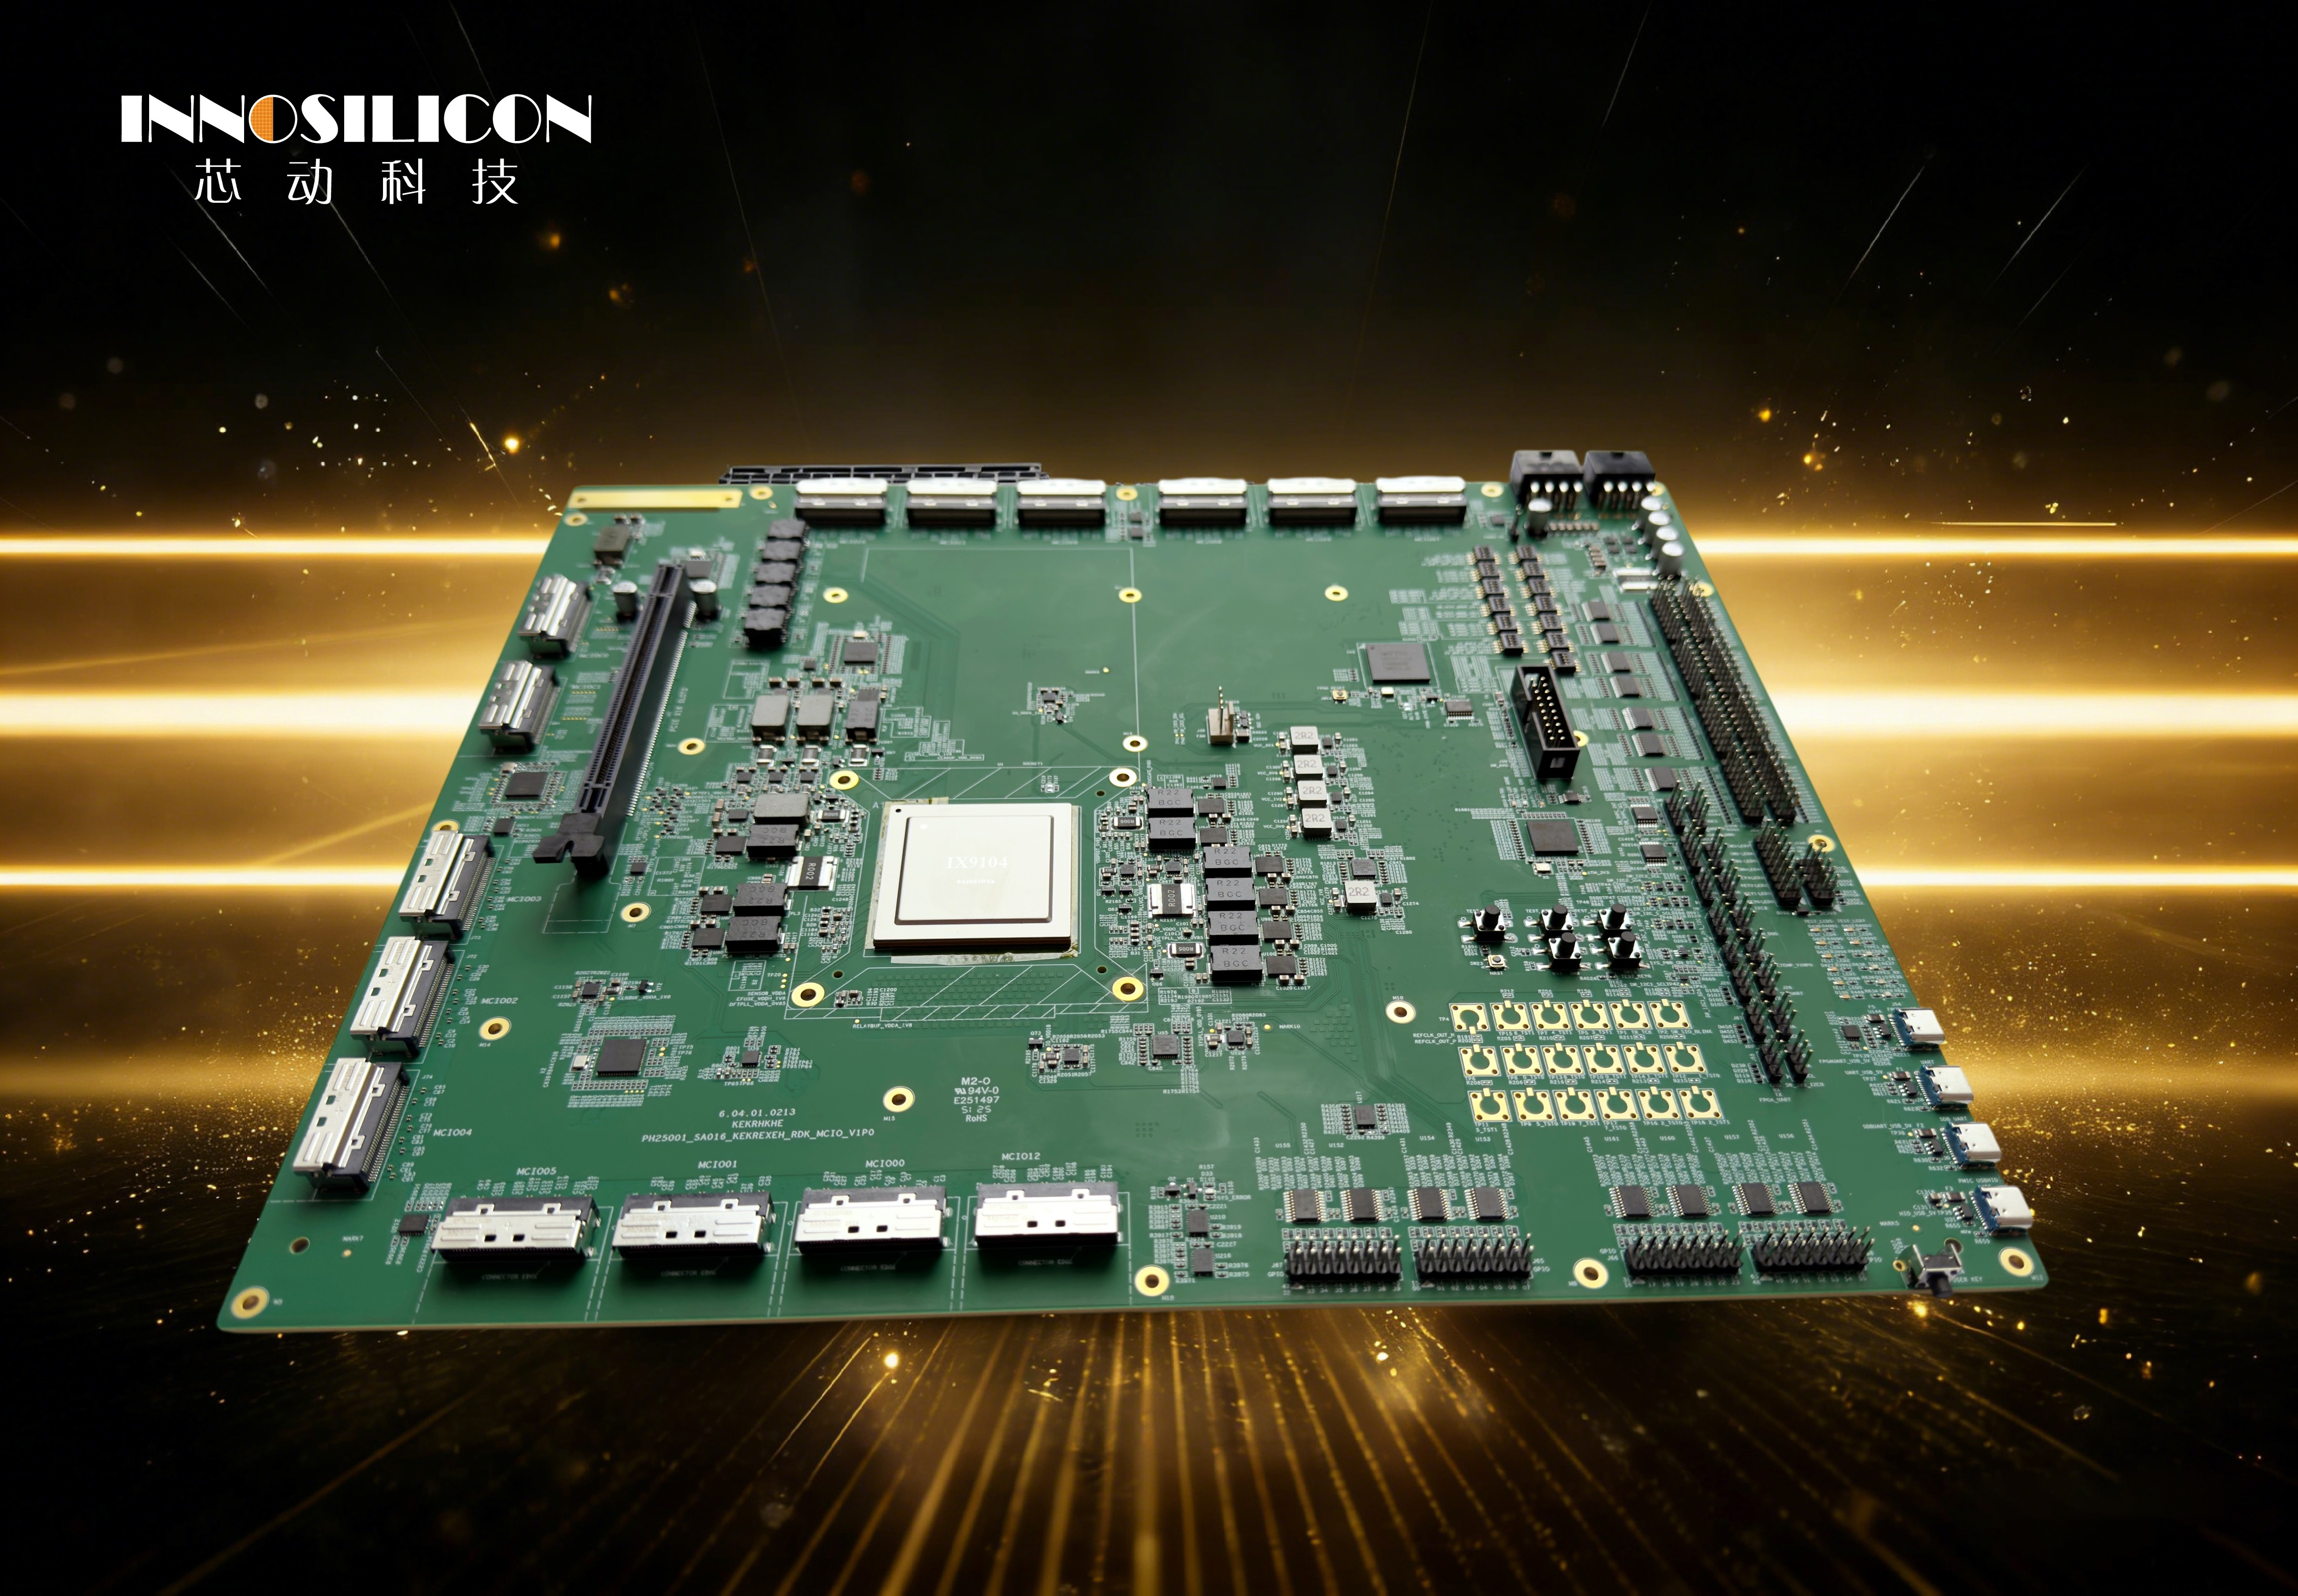
\includegraphics[width=\textwidth]{Innosilicon_new1.jpg}
      \vspace{4pt}
      {\footnotesize GX9120/GX9104 产品全景图}
    \end{column}
    \begin{column}{0.48\textwidth}
      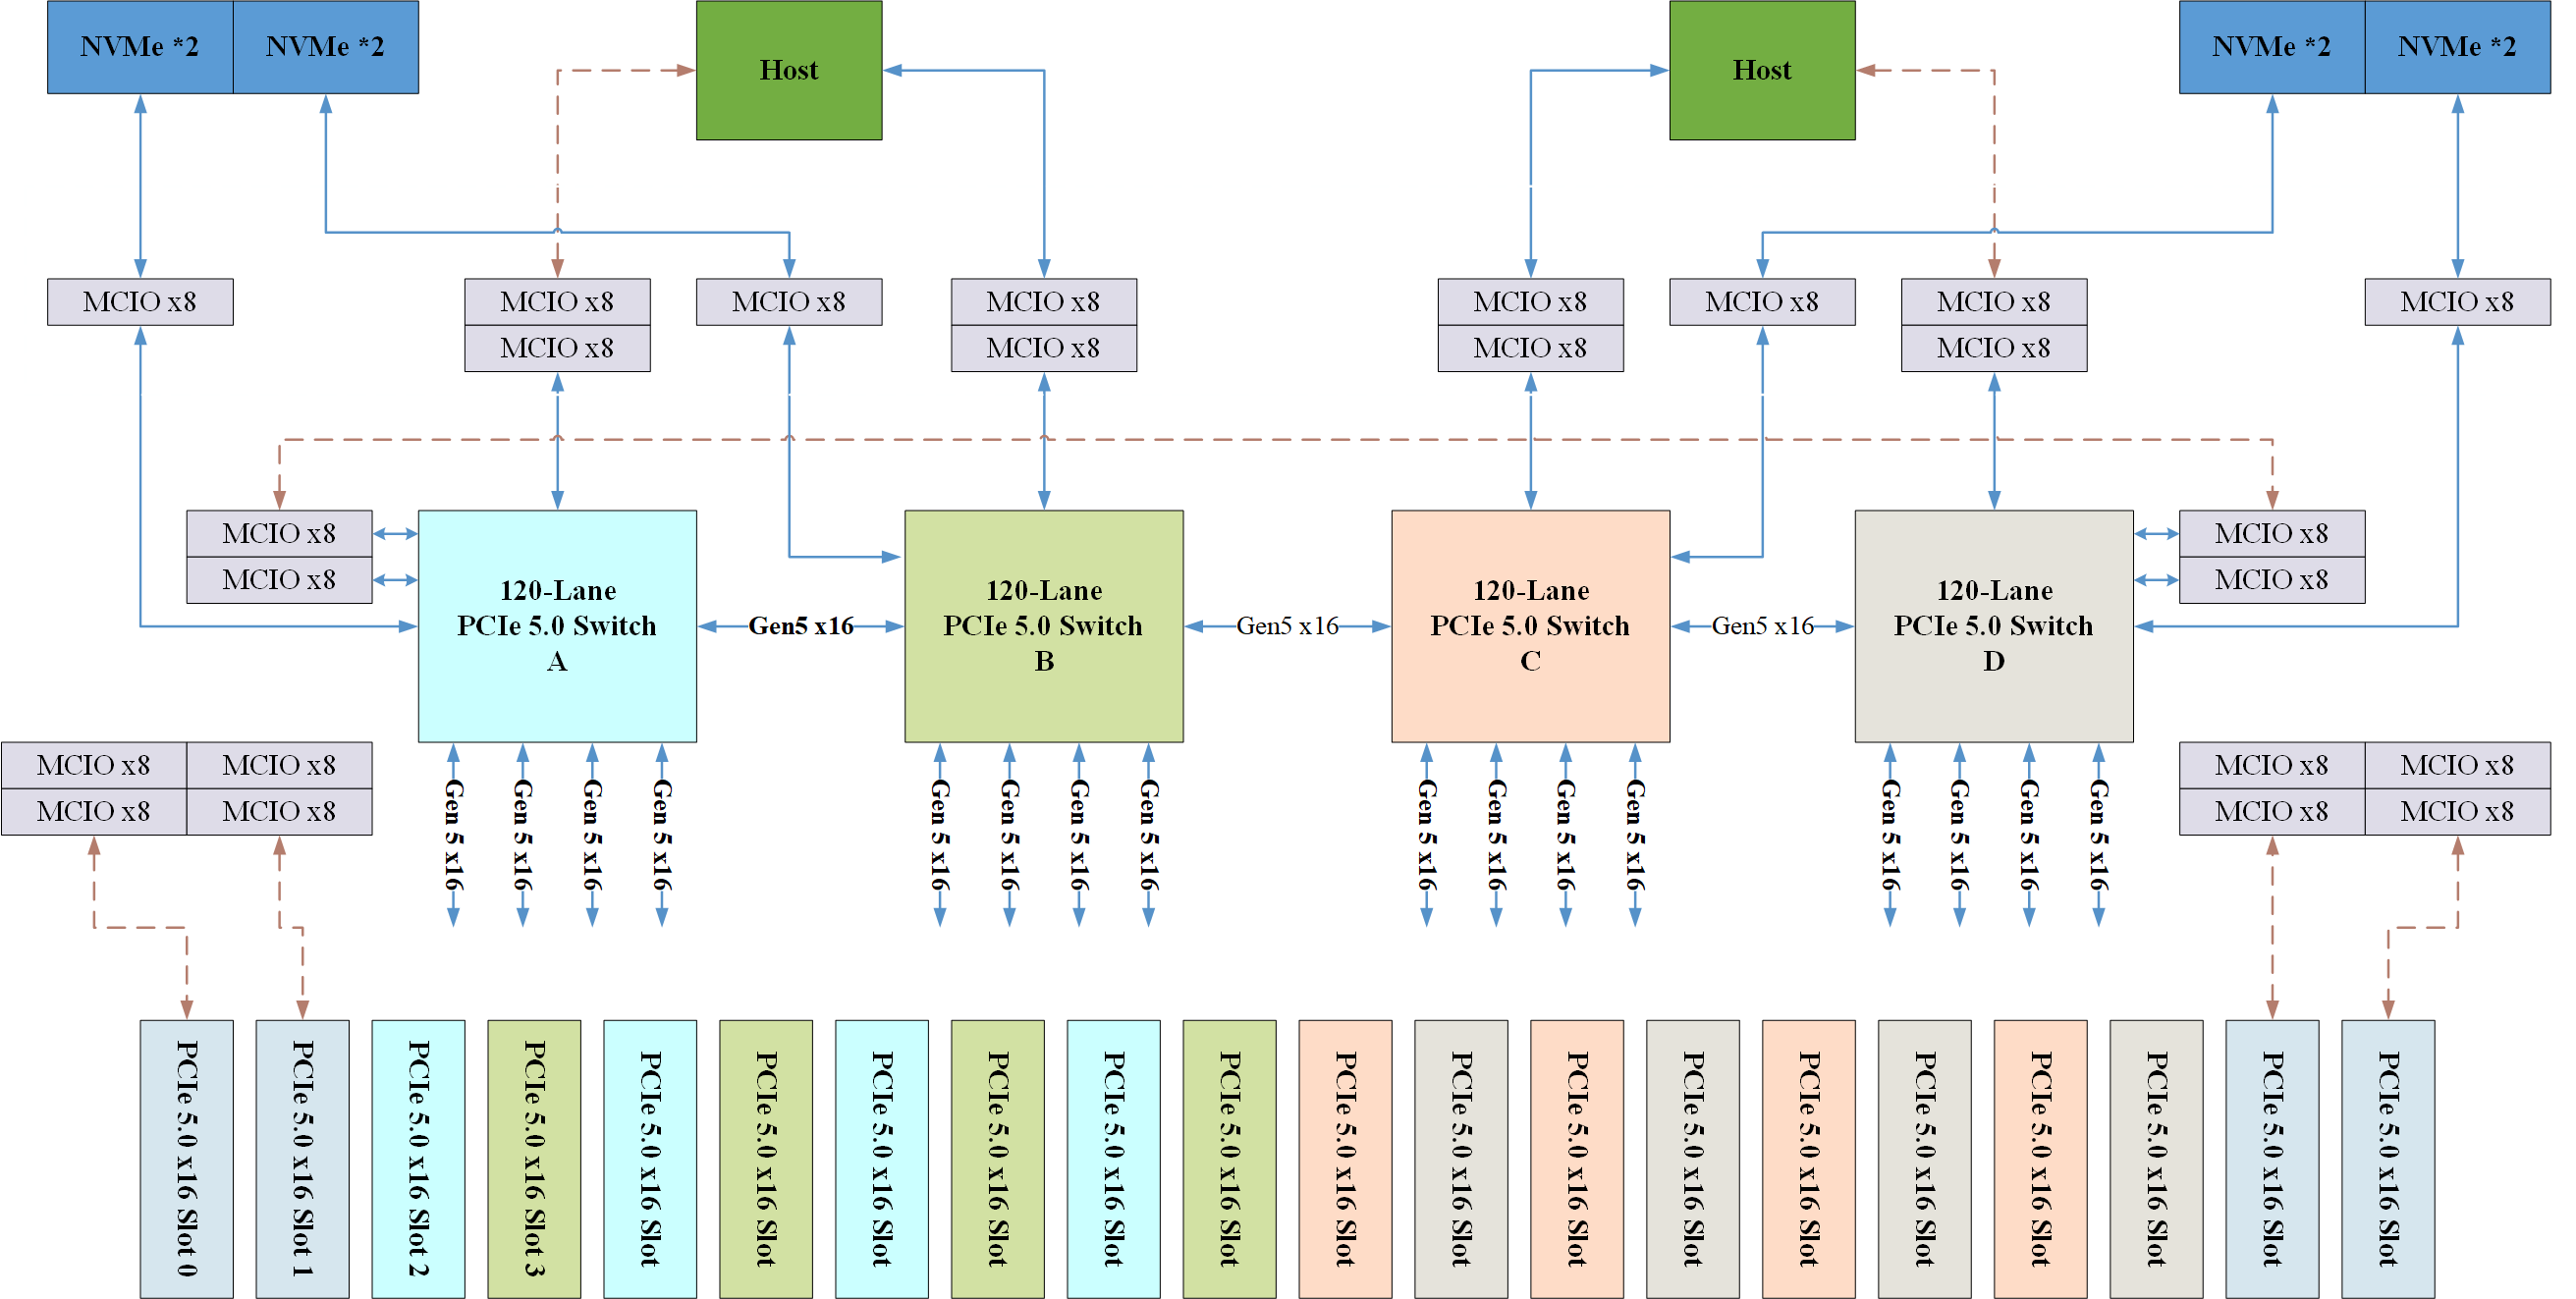
\includegraphics[width=\textwidth]{Innosilicon_screenshot.png}
      \vspace{4pt}
      {\footnotesize  16卡全互联}
    \end{column}
  \end{columns}

  \vspace{8pt}
  \begin{center}
    \textbf{120 通道 PCIe Gen5 Switch \quad$\cdot$\quad 全自研底层 IP \quad$\cdot$\quad 2026.02 武汉光谷发布}
  \end{center}
\end{frame}

\begin{frame}{代表产品对比：芯动 vs Astera vs Broadcom}
  \centering
  \footnotesize
  \begin{tabularx}{\textwidth}{p{2.2cm} X X X}
    \toprule
    \textbf{指标} & \textbf{芯动 GX9120} & \textbf{Astera Scorpio P} & \textbf{Broadcom (对标)} \\
    \midrule
    通道数     & \textbf{120}                & 32--320                  & 104 / 144 \\
    端口数     & 30 可配置                   & 全矩阵配置                 & — \\
    协议       & PCIe Gen5                  & PCIe 5.0 / CXL            & PCIe Gen5 \\
    延迟       & \textbf{115 ns}             & 超低延迟                  & — \\
    SerDes     & 14 级 DFE, 36 dB           & 自研 DSP                  & 自研 \\
    安全       & PUF + 防火墙                & Secure Boot + RoT        & — \\
    特色       & NTP 热插拔, 16 GPU          & Hypercast, In-Network Compute & — \\
    量产状态   & 2026.02 发布, 适配国产服务器  & 已量产 (P 系列)            & 已量产 \\
    自研 IP    & \textbf{全自研}底层 IP        & 自研                      & 自研 \\
    \bottomrule
  \end{tabularx}

  \vspace{6pt}
  \begin{exampleblock}{战略意义}
    芯动科技扎根底层 IP 研发近 20 年，GX9120 打破博通/微芯长期垄断。已前瞻布局 \textbf{144 通道 PCIe 6.0 / CXL 3.0 Switch} 及 PCIe 7.0 Switch。
  \end{exampleblock}
\end{frame}
% ================================================================
\section{Credo Semiconductor：全栈互联方案}
% ================================================================

\begin{frame}{Credo：AEC 发明者 \& AI 互联全栈玩家}
  \centering
  \begin{columns}[T]
    \begin{column}{0.42\textwidth}
      % 图片过大时在 column 中使用相对于列宽的缩放，避免超出布局。
      % 使用 \linewidth 以适配 column 的可用宽度。
      % 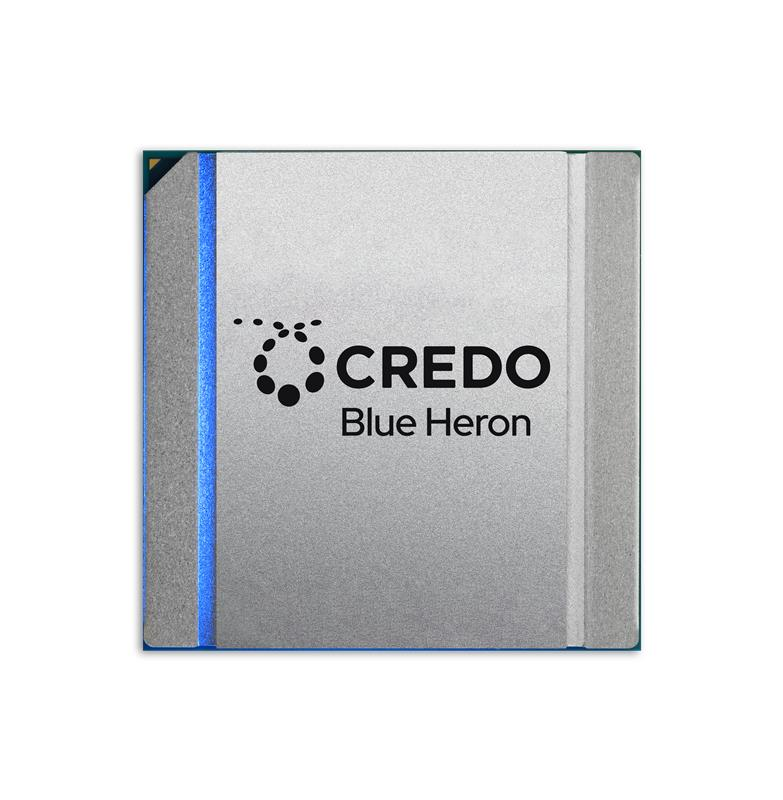
\includegraphics[width=\linewidth]{Credo_BlueHeron.jpg}
      % \vspace{6pt}
      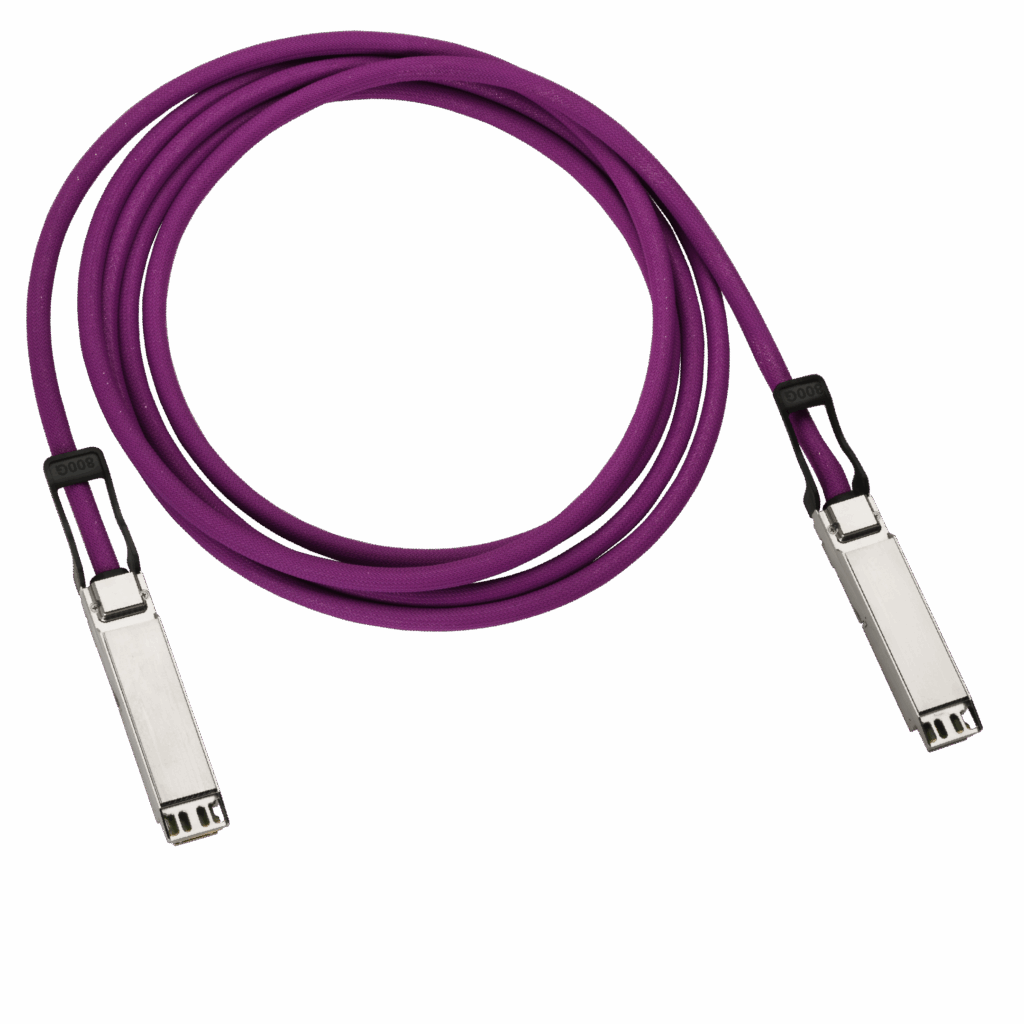
\includegraphics[width=\linewidth]{Credo_AEC.png}
    \end{column}
    \begin{column}{0.58\textwidth}
      \begin{block}{公司定位 (NASDAQ: CRDO)}
        \begin{itemize}
          \item \textbf{AEC (有源电缆) 发明者}，市占率 {\textasciitilde}\textbf{88\%}（650 Group）
          \item 自研 SerDes IP：覆盖 28G {\textasciitilde} \textbf{224G} PAM4，3nm/5nm/7nm 多节点
          \item FY2025 营收 \$4.37 亿，FY2026E {\textasciitilde}\textbf{\$9.85 亿} (+125\%)
          \item 毛利率 67.7\%，现金储备 {\textasciitilde}\$13 亿
          \item 收购 DustPhotonics (硅光) + CoMira (FEC/安全 IP)
          \item 4 家美国头部 hyperscaler 客户
        \end{itemize}
      \end{block}
      \begin{alertblock}{Blue Heron 224G — 业界首款多协议 Scale-Up Retimer}
        \textbf{3nm} 工艺，224 Gbps/通道，同时支持 \textbf{UALink + ESUN + Ethernet}。
        30-Tap FFE + 16-Tap 反射消除，\textbf{40+ dB} 链路恢复。2026.01 送样，CQ3 量产。
      \end{alertblock}
    \end{column}
  \end{columns}
\end{frame}

\begin{frame}{Credo 产品矩阵与财务}
  \centering
  \scriptsize
  \begin{tabularx}{\textwidth}{p{2.2cm} p{3.0cm} p{3.3cm} p{3.5cm}}
    \toprule
    \textbf{产品线} & \textbf{代表产品} & \textbf{核心指标} & \textbf{状态} \\
    \midrule
    \textbf{Blue Heron Retimer}
      & 224G 多协议 Retimer
      & 3nm, UALink/ESUN/Ethernet, 40+ dB
      & 2026.01 送样, CQ3 量产 \\
    \addlinespace
    \textbf{ZeroFlap AEC}
      & 有源电缆 (100G{\textasciitilde}1.6T)
      & 市占率 {\textasciitilde}88\%, 7m, 功耗降 50\%
      & 已量产, PCIe 6 AEC 送样 \\
    \addlinespace
    \textbf{Cardinal DSP}
      & 1.6T 光学 DSP
      & 3nm, 224G PAM4, EML+硅光驱动
      & 已送样 \\
    \addlinespace
    \textbf{Robin DSP}
      & 800G/400G 光学 DSP
      & 第六代架构, Full Retimed + LRO
      & 已供货 \\
    \addlinespace
    \textbf{PCIe Gen6 Retimer}
      & PCIe/CXL Retimer
      & sub 7ns, 11W, 40 dB
      & 设计赢单, FY27 贡献收入 \\
    \addlinespace
    \textbf{OmniConnect}
      & 112G VSR SerDes / Gearbox
      & 超短距, 低功耗
      & FY28 量产 \\
    \addlinespace
    \textbf{ZeroFlap Optics}
      & 800G 光收发模块
      & PILOT 链路预测, 1000×可靠性
      & 2026.03 推出 \\
    \bottomrule
  \end{tabularx}

  \vspace{-1pt}
  \begin{columns}[T]
    \begin{column}{0.48\textwidth}
      \begin{exampleblock}{财务增长轨迹}
        FY2025: \$4.37 亿 \quad FY2026E: {\textasciitilde}\$9.85 亿 \quad FY2027E: {\textasciitilde}\$13.8 亿 \\
        Q3 FY2026 单季 \$4.07 亿 (接近去年全年)
      \end{exampleblock}
    \end{column}
    \begin{column}{0.52\textwidth}
      \begin{alertblock}{战略卡位}
        AEC (铜) + Optical DSP (光) + Retimer + SerDes IP + Gearbox 五大支柱。\\
        TAM > \$100 亿，Scale-Up 组网市场 2030E > \$400 亿。
      \end{alertblock}
    \end{column}
  \end{columns}
\end{frame}

% ================================================================
\section{内存层：CXL 互联与内存池化}
% ================================================================

\begin{frame}{CXL.mem vs RDMA：数据通路的本质差异}
  \begin{columns}[T]
    \begin{column}{0.48\textwidth}
      \begin{alertblock}{RDMA：消息传递语义 (Message-based)}
        \begin{enumerate}
          \item CPU $\to$ 内存 $\to$ 组装网络包
          \item $\to$ NIC 网卡处理 QP \& Doorbell
          \item $\to$ 交换机 $\to$ NIC $\to$ 拆包
          \item $\to$ 内存 $\to$ CPU
        \end{enumerate}
        \vspace{4pt}
        \centering
        延迟：\textbf{1\textasciitilde5 \textmu s}\\[2pt]
        多级拷贝 + 协议栈开销
      \end{alertblock}
    \end{column}
    \begin{column}{0.52\textwidth}
      \begin{exampleblock}{CXL.mem：Load/Store 内存语义}
        \begin{enumerate}
          \item CPU 执行 Load/Store 指令 $\to$ Cache Miss
          \item Home Agent $\to$ CXL Root Complex 路由
          \item $\to$ CXL.mem Flit 硬件封装 (64B 缓存行)
          \item $\to$ CXL Switch 硬件路由转发
          \item $\to$ Type-3 设备内存控制器执行
          \item $\to$ 数据原路返回 CPU Cache
        \end{enumerate}
        \vspace{4pt}
        \centering
        延迟：\textbf{100\textasciitilde300 ns}\\[2pt]
        零网卡、零拆包、零协议栈
      \end{exampleblock}
    \end{column}
  \end{columns}

  \vspace{6pt}
  \begin{block}{核心本质}
    CXL 将以往只存在于主板上的\textbf{「总线拓扑」}强行拉伸到机架甚至数据中心规模。RDMA 是网络消息，CXL 是\textbf{硬件状态机直飞}。
  \end{block}
\end{frame}

\begin{frame}{物理走线：机架内 vs 跨机柜}
  \begin{columns}[T]
    \begin{column}{0.48\textwidth}
      \begin{block}{机架内 (Intra-Rack)：1\textasciitilde3 米}
        \textbf{电信号方案：Retimer + AEC 铜缆}
        \begin{itemize}
          \item \textbf{DAC / MCIO}：极短距直连
          \item \textbf{AEC 有源电缆}：两端内置 Retimer 芯片（CDR + FFE/DFE 均衡），将劣化 PAM4 信号重新整形放大
          \item \textbf{代表方案}：Astera Labs Aries + Taurus，澜起 M88RT61632 + AEC 方案
        \end{itemize}
      \end{block}
    \end{column}
    \begin{column}{0.52\textwidth}
      \begin{alertblock}{跨机柜 (Inter-Rack)：3 米以上}
        \textbf{光互连方案：CXL over Optics}
        \begin{itemize}
          \item \textbf{CPO (光电共封装)}：硅光引擎与 CXL Switch 封装在同一基板，消除面板光模块延迟
          \item \textbf{LPO (线性直驱)}：去掉光模块 DSP，CXL 时钟直接驱动光器件，压缩 {\textasciitilde}数十 ns 延迟
          \item \textbf{全光走线}：MPO/MTP 单模光纤，CXL 协议运行在光信道上
          \item \textbf{代表方案}：Ayar Labs TeraPHY，阿里云 LPO + CXL
        \end{itemize}
      \end{alertblock}
    \end{column}
  \end{columns}

  \vspace{6pt}
  \begin{center}
    \textbf{短距死磕电信号极限 (Retimer + AEC) \quad$\longrightarrow$\quad 远距依靠硅光互连 (CXL over Optics)}
  \end{center}
\end{frame}

\begin{frame}{CXL 内存池化：业界代表案例}
  \centering
  \footnotesize
  \begin{tabularx}{\textwidth}{p{3.2cm} p{3.2cm} p{3.0cm} p{4.5cm}}
    \toprule
    \textbf{厂商} & \textbf{产品/方案} & \textbf{物理实现} & \textbf{数据通路关键点} \\
    \midrule
    \textbf{Astera Labs}
      & Leo CXL 内存控制器 + Aries Retimer
      & AEC 线缆 + E3.S 内存扩展模块
      & Retimer CDR 恢复 PAM4 信号，无损传至 JBOM 内存池 \\
    \addlinespace
    \textbf{Samsung / SK Hynix}
      & CMM-D / CXL 内存模块
      & E3.S 热插拔 + 自研 CXL 控制器 + DDR5
      & CXL Flit 直接译为 DDR5 RAS/CAS，完全旁路网络栈 \\
    \addlinespace
    \textbf{UnifabriX}
      & CXL 3.0 Smart Memory Node
      & 2U 独立硬件 + CXL Switch + 大容量内存条
      & Switch 硬件路由 + Fabric Manager 动态重分配内存（秒级） \\
    \addlinespace
    \textbf{Ayar Labs}
      & TeraPHY 光学 I/O 芯粒 (CPO)
      & 硅光 Chiplet 与 CPU/Switch 同基板封装
      & 电信号 $\to$ 几毫米内转光 $\to$ 单模光纤跨 50m 机柜 \\
    \addlinespace
    \textbf{阿里云}
      & 磐久 CXL + LPO 直驱光模块
      & LPO 去 DSP 光模块 + 自研 CXL 控制器
      & CXL 时钟直接驱动光器件，省 DSP 延迟 {\textasciitilde}数十 ns \\
    \bottomrule
  \end{tabularx}

  \vspace{6pt}
  \begin{exampleblock}{层级划分}
    \textbf{机架内 (铜)}：Astera / Samsung / SK Hynix 已量产商用 \quad \\
    \textbf{系统级池化}：UnifabriX 展示动态切分 \quad \\
    \textbf{跨机柜 (光)}：Ayar / 阿里云 指明终局形态
  \end{exampleblock}
\end{frame}



% ================================================================
\section{横向对比：全产品线竞争力评估}
% ================================================================

\begin{frame}{全产品线竞争力矩阵}
  \centering
  \footnotesize
  \begin{tabularx}{\textwidth}{p{2.4cm} c c c c c p{2.2cm}}
    \toprule
    \textbf{产品线} & \textbf{技术} & \textbf{市场} & \textbf{壁垒} & \textbf{团队} & \textbf{时机} & \textbf{综合} \\
    & \textbf{成熟度} & \textbf{空间} & \textbf{高度} & \textbf{匹配度} & \textbf{窗口} & \textbf{评级} \\
    \midrule
    Retimer / Smart Cable
      & $\star$$\star$$\star$$\star$ & $\star$$\star$$\star$$\star$$\star$ & $\star$$\star$$\star$$\star$ & $\star$$\star$$\star$$\star$ & $\star$$\star$$\star$$\star$$\star$ & \textbf{A} \\
    \addlinespace
    Smart Switch
      & $\star$$\star$$\star$ & $\star$$\star$$\star$$\star$ & $\star$$\star$$\star$$\star$$\star$ & $\star$$\star$$\star$ & $\star$$\star$$\star$$\star$ & \textbf{B+} \\
    \addlinespace
    CXL 内存控制器
      & $\star$$\star$$\star$ & $\star$$\star$$\star$$\star$ & $\star$$\star$$\star$$\star$ & $\star$$\star$$\star$$\star$ & $\star$$\star$$\star$$\star$ & \textbf{A-} \\
    \addlinespace
    SuperNIC
      & $\star$$\star$$\star$ & $\star$$\star$$\star$$\star$ & $\star$$\star$$\star$$\star$$\star$ & $\star$$\star$$\star$ & $\star$$\star$$\star$ & \textbf{B} \\
    \addlinespace
    D2D PHY IP
      & $\star$$\star$$\star$ & $\star$$\star$$\star$$\star$ & $\star$$\star$$\star$$\star$ & $\star$$\star$ & $\star$$\star$$\star$ & \textbf{B} \\
    \addlinespace
    硅光 / CPO
      & $\star$$\star$ & $\star$$\star$$\star$$\star$$\star$ & $\star$$\star$$\star$$\star$$\star$ & $\star$$\star$ & $\star$$\star$ & \textbf{B+} \\
    \bottomrule
  \end{tabularx}
\end{frame}

\begin{frame}{关键差异化维度对比}
  \centering
  % 示例：雷达图 / 气泡图
\end{frame}

% ================================================================
\section{供应链与生态分析}
% ================================================================

\begin{frame}{关键供应链环节}
  \begin{columns}[T]
    \begin{column}{0.50\textwidth}
      \begin{block}{上游依赖}
        \begin{itemize}
          \item \textbf{SerDes IP}：核心壁垒，澜起自研掌握
          \item \textbf{晶圆代工}：成熟制程 (16/12/7nm)，不依赖最先进节点
          \item \textbf{封装}：FCCSP 业界主流，不依赖 CoWoS 先进封装
          \item \textbf{测试设备}：Keysight / Tektronix / Viavi，PCIe 6.0 验证复杂度指数上升
        \end{itemize}
      \end{block}
    \end{column}
    \begin{column}{0.50\textwidth}
      \begin{exampleblock}{下游客户}
        \begin{itemize}
          \item \textbf{云厂商}：国内头部 CSP (阿里/腾讯/字节)
          \item \textbf{服务器 OEM}：浪潮/新华三/联想
          \item \textbf{GPU/AI 芯片厂商}：国产 GPU 互联需求
          \item \textbf{线缆/模块厂商}：AEC 有源线缆集成
        \end{itemize}
      \end{exampleblock}
    \end{column}
  \end{columns}

  \vspace{8pt}
  \begin{alertblock}{关键判断}
    Retimer 产品不依赖最先进制程和先进封装，\textbf{供应链风险可控}；核心瓶颈在 SerDes IP 和互操作性验证。
  \end{alertblock}
\end{frame}

\begin{frame}{主要并购与融资事件}
  \centering
  \footnotesize
  \begin{tabularx}{\textwidth}{p{3.0cm} p{3.0cm} p{2.8cm} p{3.5cm}}
    \toprule
    \textbf{事件} & \textbf{金额} & \textbf{时间} & \textbf{战略意图} \\
    \midrule
    Marvell 收购 XConn
      & \$5.4 亿      & 2026        & 混合交换芯片 (Apollo 2)，打造开放 Fabric \\
    \addlinespace
    Marvell 收购 Celestial AI
      & \$32.5 亿     & 2026        & 光子 Fabric 技术，挑战 NVLink 生态 \\
    \addlinespace
    Ayar Labs E 轮
      & \$5 亿        & 2026.03     & CPO 光引擎量产，估值 \$37.5 亿 \\
    \addlinespace
    Enfabrica C 轮
      & \$1.15 亿     & 2026        & SuperNIC ACF-S 芯片，3.2 Tbps \\
    \addlinespace
    Eliyan 战略融资
      & \$5000 万     & 2025        & 标准封装 D2D，AMD/ARM/Samsung 参投 \\
    \bottomrule
  \end{tabularx}
\end{frame}

% ============================================
%  结束页
% ============================================
\begin{frame}[plain]
  \centering
  \vfill
  {\huge\color{ieeeBlue} 谢谢！欢迎提问}

  \vspace{20pt}
  {\large 葛良晨}

  \vspace{8pt}
  {\large \today}
  \vfill
\end{frame}

\end{document}
